%\documentclass[aps,prl,preprint]{revtex4-1}
\documentclass[aps,prb,showpacs,preprintnumbers,amsmath,amssymb,superscriptaddress,twocolumn]{revtex4-1}
\usepackage{graphicx}
\usepackage{comment}
%\usepackage[caption=false]{subfig}
%\usepackage{subcaption}
%\captionsetup[subfigure]{labelformat=brace}
\usepackage{hyperref}
\usepackage{braket}

\newcommand{\midrule}{\hline}
\newcommand{\bottomrule}{\hline\hline}
\newcommand{\bs}{\boldsymbol}
\newcommand{\tr}{\text{tr}}

\usepackage{xcolor}

\graphicspath{{./figures/}}

\newcommand{\up}{\uparrow}
\newcommand{\down}{\downarrow}
\newcommand{\david}[1]{ \textcolor{red}{\textbf{DC: #1}}}
\newcommand{\mh}[1]{ \textcolor{blue}{\textbf{#1}}}


\usepackage{esint}
\makeatletter
%% make esint definition in line with amsmath
\@for\next:={int,iint,iiint,iiiint,dotsint,oint,oiint,sqint,sqiint,
  ointctrclockwise,ointclockwise,varointclockwise,varointctrclockwise,
  fint,varoiint,landupint,landdownint}\do{%
    \expandafter\edef\csname\next\endcsname{%
      \noexpand\DOTSI
      \expandafter\noexpand\csname\next op\endcsname
      \noexpand\ilimits@
    }%
  }
\makeatother

\begin{document}
\title{Quantum Monte Carlo Compton profiles of solid and liquid lithium}
\author{Yubo Yang}
\affiliation{Department of Physics, University of Illinois, Urbana, Illinois 61801, USA}
\author{Nozomu Hiraoka}
\affiliation{National Synchrotron Radiation Research Center, Hsinchu 30076, Taiwan}
\author{Kazuhiro Matsuda}
\affiliation{Graduate School of Science, Kyoto University, Kyoto 606-8502, Japan}
\author{Markus Holzmann}
\affiliation{Univ. Grenoble Alpes, CNRS, LPMMC, 38000 Grenoble, France}
\affiliation{Institut Laue Langevin, BP 156, F-38042 Grenoble Cedex 9, France}
\author{David M. Ceperley}
\affiliation{Department of Physics, University of Illinois, Urbana, Illinois 61801, USA}
\date{\today}
\begin{abstract}
We computed the Compton profile of solid and liquid lithium using quantum Monte Carlo (QMC) and compared with recent experimental measurements obtaining good agreement. Importantly, we find it crucial to account for proper core-valence orthogonalization and to address density differences when comparing to experiment. To account for disorder effects, we sampled finite-temperature configurations using molecular dynamics (MD), then performed diffusion Monte Carlo (DMC) simulations on each configuration. We used Slater-Jastrow wavefunctions and grand-canonical twist-averaged boundary conditions. A QMC pseudopotential correction, derived from an all-electron DMC simulation of the perfect crystal was also used. Our calculations provide the first all-electron QMC benchmark for the Compton profile of lithium crystal and pseudopotential-corrected QMC Compton profiles for both the liquid and solid.
\end{abstract}
\pacs{}
\maketitle

\section{Introduction} \label{sec:intro}

The Compton profile is a bulk-sensitive probe of the electronic structure of a material accessible to both theory and experiment. Using the ``impulse approximation''~\cite{Eisenberger1970}, the double differential cross section of inelastic light scattering is directly proportional to the Compton profile, the Radon transform of the electronic momentum distribution along the scattering vector. %The directional Compton profile along z is
\begin{equation}
J(p_z) = \iint dk_x dk_y ~ n(k_x, k_y, k_z=p_z),
\end{equation}
where $n(\bs{k})$ is the electronic momentum distribution.
Since the pioneering work of Eisenberger et. al.~\cite{Eisenberger1970,Eisenberger1972}, Compton scattering experiments have been performed on simple metals such as Li~\cite{Sakurai1995, Schulke1996,Chen1999,Sternemann2001,Tanaka2001}, Be~\cite{Hamalainen1996,Huotari2000}, Na~\cite{Huotari2010} as well as more complicated materials. Accompanying the scattering experiments are numerous theoretical calculations using different electronic structure theories including density functional theory (DFT)~\cite{Sakurai1995,Schulke1996,Tanaka2001,Jarlborg1998,Baruah1999,Bross2005,Makkonen2005,Klevak2016,Sekania2018}, QMC~\cite{Filippi1999,Huotari2010}, and GW~\cite{Yasunori1997,Schulke1999,Eguiluz2000,Olevano2012}.
The Compton profiles in ref.~\cite{Sakurai1995,Schulke1996} were compared to DFT results using the local density approximation (LDA) with the Lam-Platzman correlation correction~\cite{Lam1974}.
While the Lam-Platzman correction has been shown to be accurate by QMC~\cite{Filippi1999,Schulke2001,Bross2005}, the theoretical Compton profile is still larger at low momenta and smaller at high momenta compared with experiment. In other words, the predicted Compton profile is typically narrower than observed.

Both theoretical approximations and experimental procedures may be responsible for a significant fraction of the aforementioned discrepancy. In the experiment, finite momentum resolution and final-state effects~\cite{Sternemann2000,Soininen2001} broaden the measured Compton profile. In the theory side, the lack of electronic correlation and the use of pseudopotentials both narrow the computed Compton profile. Furthermore, many subtle complications may also be responsible for part of the discrepancy. Examples include: multiple scattering corrections, background subtraction, thermal expansion, electron-phonon coupling, and relativistic effects.

In this paper, we present much improved QMC calculations on the solid and the liquid state of lithium. Firstly, we use grand-canonical twist-averaging~\cite{Lin2001} to access the momentum distribution at arbitrary momentum while preserving a sharp Fermi surface. We obtain a momentum resolution of 0.040 a.u., which is higher than the 0.068 a.u. achieved previously~\cite{Filippi1999} (It is straight-forward to further increase momentum resolution given more computational resources). Secondly, we perform Diffusion Monte Carlo (DMC) to remove effects of the trial wavefunction. Thirdly, we use all-electron QMC to explore the pseudopotential bias in the Compton profile. We find that the pseudopotential bias is responsible for the majority of discrepancy between pseudopotential QMC and experimental Compton profiles away from the Fermi surface. Fourth and finally, we apply finite-size corrections~\cite{Holzmann2009,Holzmann2011} to obtain the momentum distribution in the thermodynamic limit. Using these improved procedures, we calculate the disorder-averaged Compton profiles for polycrystal and liquid lithium and obtain good agreement with recent high-resolution synchrotron experiment [N. Hiraoka and K. Matsuda].

This paper is organized as follows. In section \ref{sec:method}, we describe the simulation methods used to obtain the QMC momentum distributions. In section \ref{sec:results}, we show the QMC momentum distributions and the resulting Compton profiles in comparison with experiment. In section \ref{sec:discussion}, we discuss the influence of various physical effects on the momentum distribution in an attempt to explain the remaining discrepancy between QMC and experiment.

\section{Method} \label{sec:method}

Full-core and pseudopotential QMC calculations have been performed on both  the perfect crystal and disordered lithium configurations. %All QMC calculations use the Slater-Jastrow trial wavefunction eq.~(\ref{eq:sj})  
We use Slater-Jastrow trial wavefunction
\begin{align}
\Psi_T = D^{\up} D^{\down} \exp\left[ -\sum\limits_{i<j}^{N} u(\bs{r}_i-\bs{r}_j) - \sum\limits_{i=1}^N \chi(\bs{r}_i) \right],\label{eq:sj}
\end{align}
where $u(\bs{r})$ is the electron-electron Jastrow pair function, $\chi(\bs{r})$ is the electron-ion Jastrow pair function and $\bs{r}_i$ is the position of the i$^{th}$ electron. The Slater determinant $D^{\up/\down}$ is composed of single-particle orbitals obtained using Kohn-Sham (KS) DFT with the LDA functional. In the full-core calculation, we remove the approximate electron-ion cusp from the orbitals and re-introduce the exact cusp condition in the Jastrow function~\cite{Ceperley1981}. In the pseudopotential calculation, we treat the lithium atoms as pseudo ions of charge +1. The core, screened by 1s electrons, is replaced by the BFD pseudopotential~\cite{Burkatzki2007}.  The electron-electron Jastrow pair function is expressed as a sum of real-space and reciprocal space parts to accurately describe long-range plasmon fluctuations.

In variational Monte Carlo (VMC), we sample $\vert \psi_T \vert^2$ using Metropolis Monte Carlo and directly calculate properties from the many-body wavefunction. The momentum distribution is calculated using the direct estimator in reciprocal space\cite{W.L.McMillan1965}. In DMC, an ensemble of electron configurations evolve according to the Green's function of the non-relativistic Schr\"odinger equation in imaginary time. Using the magnitude of the trial wavefunction $\vert \psi_T\vert$ as guiding function and phase, the long-time solution samples the mixed distribution $\psi^*_T\psi_{FP}$, in the limit of small time step. $\psi_{FP}$ is the fixed-phase ground-state wavefunction. If the phase of $\psi_T$ were exact, then $\psi_{FP}$ would be the exact ground-state wavefunction.~\cite{Ortiz1993} The difference between the expectation value of an observable in the fixed-phase and the mixed distributions is the mix-estimator bias. We gauge simulation quality by monitoring kinetic, potential, and total energies as well as pair correlation functions and the momentum distribution. We observe fast equilibration, small variance and small mixed-estimator bias in all monitored quantities. The DMC momentum distribution is linearly extrapolated to remove the mixed-estimator bias. For more details on the computational methods and data processing, see the supplementary materials.

We use GCTABC to improve the momentum distribution \cite{PhysRevLett.97.076404,Holzmann2009}. A previous QMC calculation~\cite{Filippi1999} used real wavefunctions and canonical twist average boundary condition (CTABC); each boundary condition (twist) had the same number of electrons. Use of real trial functions restricted the accessible momenta to those commensurate with the simulation cell. CTABC can occupy states outside of the Fermi surface at certain twists, which artificially smears the Fermi surface. In contrast, the grand-canonical twist average technique enforces constant chemical potential at all twists. We adjusted the number of electrons at each twist such that no state outside the Fermi surface was occupied. This allows us to sample the momentum distribution at momenta arbitarily close to the Fermi surface while maintaining a sharp Fermi surface. \mh{In practice, we impose the occupation of the orbitals in the Slater determinant according to the LDA Fermi energy}. In principle, one might modify the Fermi surface by estimating the chemical potential directly within QMC \cite{yang2019electronic}. However, this is much more computationally demanding and is beyond the scope of the current study and not thought to be necessary for lithium.

In the perfect crystal, the full-core simulation contains 54 lithium atoms, while the pseudopotential simulations contain 54 or 432 atoms. We use MD with the modified embedded-atom potential (MEAM)~\cite{Baskes1992} to generate the disordered configurations.  The MD temperatures were elevated to model quantum fluctuations of the nuclei ~\cite{Filippi1998}. We sample the canonical distribution with 432 lithium atoms at 330K and 500K for experiments at 298K and 493K, respectively.

All calculations have been performed at the same density $r_s=3.25$, consistent with the previous QMC study~\cite{Filippi1999}. After obtaining QMC results at $r_s=3.25$, we rescale the density of QMC Compton profiles to match the experimental densities: $r_s=3.31$ for the liquid and $r_s=3.265$ for the solid. 

\mh{MH: Maybe we should add a short paragraph how we/the experiment determines the valence electron Compton profile already here?}

We convolved our QMC Compton profile with a broadening function to model the instrument resolution and final-state interaction. For this we used the \emph{extended Lorentzian}
\begin{equation}
b(x) = \frac{1}{\tilde{\Omega}} \frac{1}{
a_0+a_1(\frac{2x}{\Gamma})^2+a_2(\frac{2x}{\Gamma})^4
}\label{eq:elorentz}
\end{equation}
with $\Gamma=0.024$ a.u., $a_0=1$, $a_1=0.85$ and $a_2=0.15$ chosen to fit the convolution of the elastic line in the X-ray experiment and the spectral density function of the electrons and $\tilde{\Omega}$ such that $\int dx ~b(x)=1$. 

We used LAMMPS~\cite{Plimpton1993} for the MD simulations, QE~\cite{Giannozzi2009,Enkovaara2017} for the DFT, PySCF~\cite{PYSCF} for Hartree-Fock (HF), and QMCPACK~\cite{Kim2018} for QMC. The disordered calculations have been automated using the nexus suite of tools~\cite{Krogel2016}.

\section{Results} \label{sec:results}

Figure ~\ref{fig:sl-jp-djp} shows the valence Compton profiles of solid and liquid lithium from experiment and processed QMC data. The raw QMC data have been processed to account for finite-size effects, thermal disorder, pseudopotential bias, density rescaling, final-state effects, and instrument resolution. The QMC Compton profiles agree with experiment immediately inside the Fermi surface (0.2 a.u.$<$p$<$0.4 a.u.) and at large momenta (p$>$0.9  a.u.). However, the QMC Compton profiles show less high-momentum component immediately outside the Fermi surface and too much low-momentum component. Both the theoretical and experimental Compton profiles satisfy the normalization sum rule ($\int_{-\infty}^{\infty} J(p)dp=1$) to better than 0.5\%. The difference between QMC and experiment Compton profiles can be interpreted as a shift of momentum density from zero to slightly above the Fermi momentum. 

\begin{figure}[h]
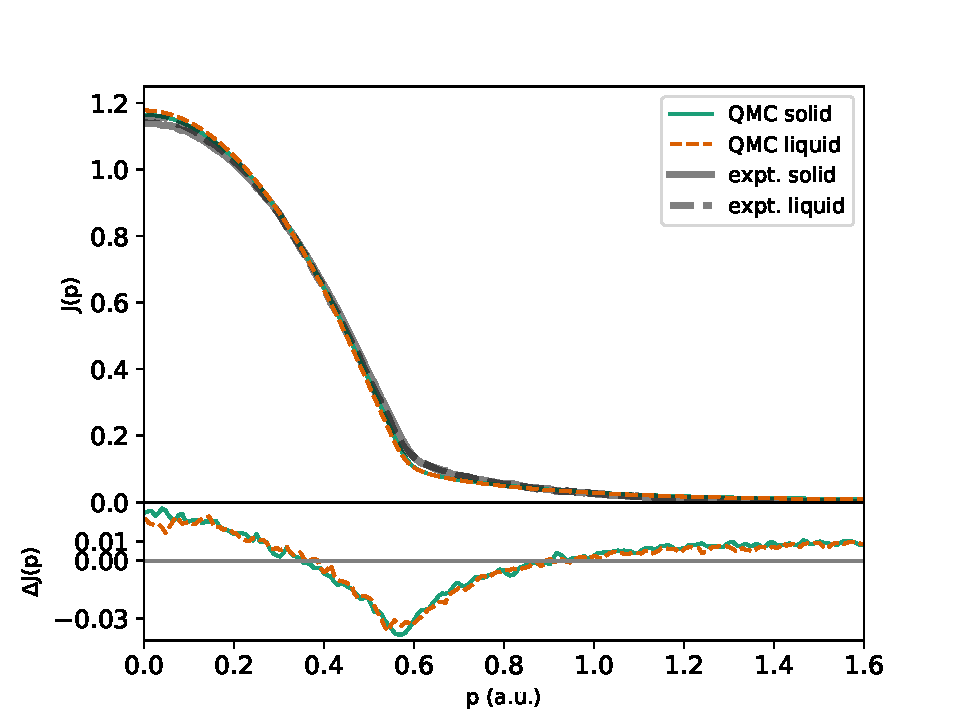
\includegraphics[width=\linewidth]{li58_sl-jp}
\caption{\mh{Valence electron} Compton profiles of solid (solid line) and liquid (dashed line) lithium from QMC (thin) and experiment (thick). The top panel shows the Compton profiles on an absolute scale. The bottom panel shows  $\Delta J(p)=J_{QMC}-J_{exp}$.}%the QMC Compton profiles relative to the experiment.
\label{fig:sl-jp-djp}
\end{figure}

Figure ~\ref{fig:s-l-djp} shows the change of the Compton profile when the liquid freezes into a solid. The systematic difference  between QMC calculations and experiment is almost identical in the solid and the liquid. Thus, cancellation of error allows us to capture the difference between the solid and liquid Compton profiles almost perfectly.
The main change is a density-induced outward shift of the Fermi surface. This shift manifests in Fig.~\ref{fig:s-l-djp} as a peak at the solid Fermi momentum $p_F\approx0.578$ a.u. and a parabolic dip centered around $p=0$. Another important difference is the emergence of secondary Fermi surfaces, due to Umklapp scattering in the solid. We expect secondary Fermi surfaces to center around the reciprocal lattice of the lithium crystal. Crystalline lithium is BCC with a lattice constant of $\sim 6.63$ bohr, so its reciprocal lattice is FCC with a lattice constant of $\sim 1.895$ a.u.. The nearest neighbor to $\Gamma$ is $p_1=1.34$ a.u.  along [110]. Therefore, the closest secondary Fermi surface is located at $p_1-p_F=0.762$ a.u., which is exactly where we observe a small peak \mh{(MH: is in't it the zero between the small negative and positive peak?)} in Fig.~\ref{fig:s-l-djp}.

\begin{figure}[h]
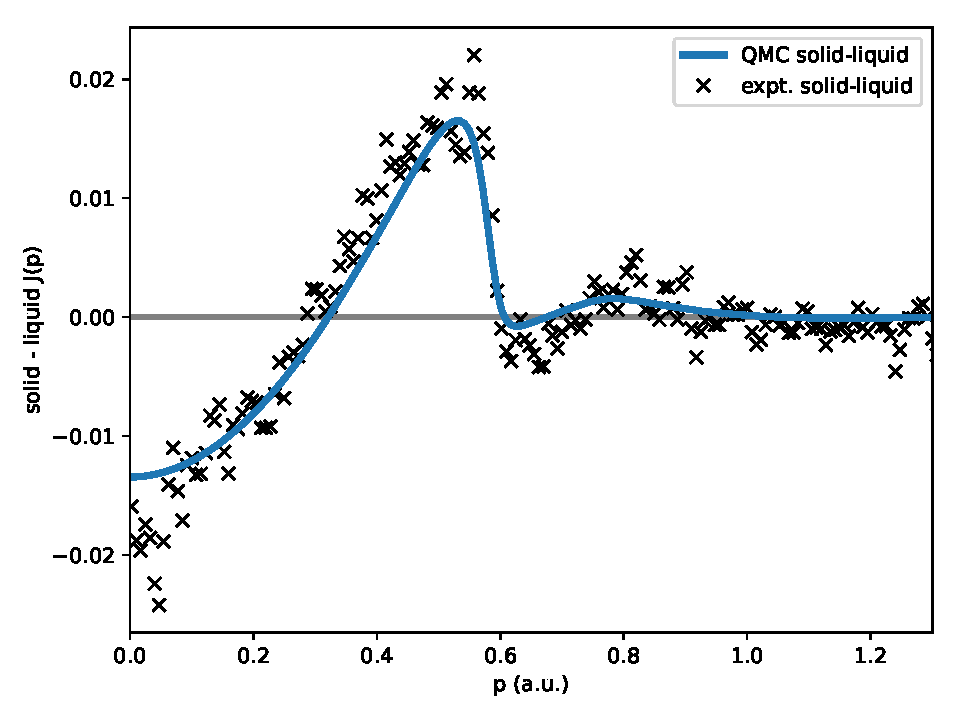
\includegraphics[width=\linewidth]{li52e_sl-djp}
\caption{Difference between solid and liquid \mh{valence electron} Compton profiles.\label{fig:s-l-djp}}
\end{figure}

As mentioned in the beginning of this section, we process the raw QMC data in several steps to make them comparable to experiment. In the following, we present perfect lithium crystal QMC calculations, which we use to validate the processing steps.

In Fig.~\ref{fig:nk}, 1D slices of the QMC valence momentum distributions are shown. The momentum distribution is free-electron-like along the [100] and [111] directions. Along the [110] direction, however, there is a pronounced secondary Fermi surface. The valence profile from the full-core calculation is flatter inside the Fermi surface and has enhanced secondary features when compared to the pseudopotential calculation. 

To obtain the valence momentum distribution from the full-core QMC calculation (red lines), we remove the momentum distribution of the 1s core electrons. The 1s orbital of the neutral lithium atom is calculated using Hartree-Fock (HF) with a cc-pV5Z basis. The most pronounced effect of the pseudopotential is to increase the electronic momentum density inside the Fermi surface, raising $n(0)$ by more than 5\%. In contrast, the effect of increasing system size peaks at the Fermi momentum. The main effect of finite system size is to increase the magnitude of the discontinuity at the Fermi momentum. The effects of pseudopotential and finite system size can be better shown in the momentum distribution differences.

\begin{figure}[h]
\begin{minipage}{\columnwidth}
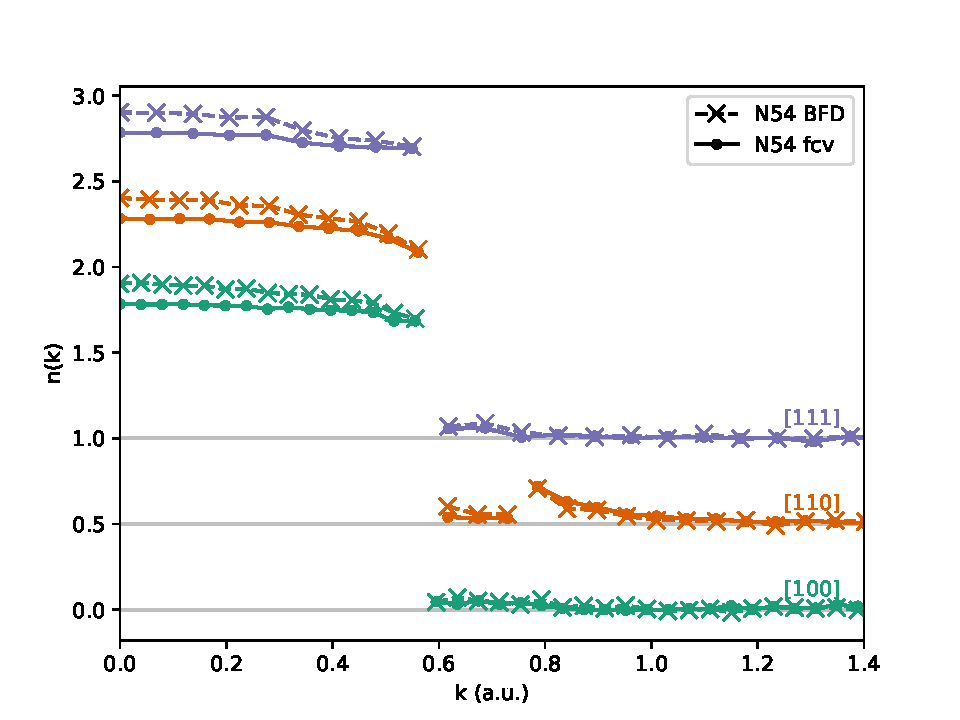
\includegraphics[width=\linewidth]{li57_dmcfc-fcv-dir}
(a) full-core valence \textit{vs} pseudopotential
\end{minipage}
\begin{minipage}{\columnwidth}
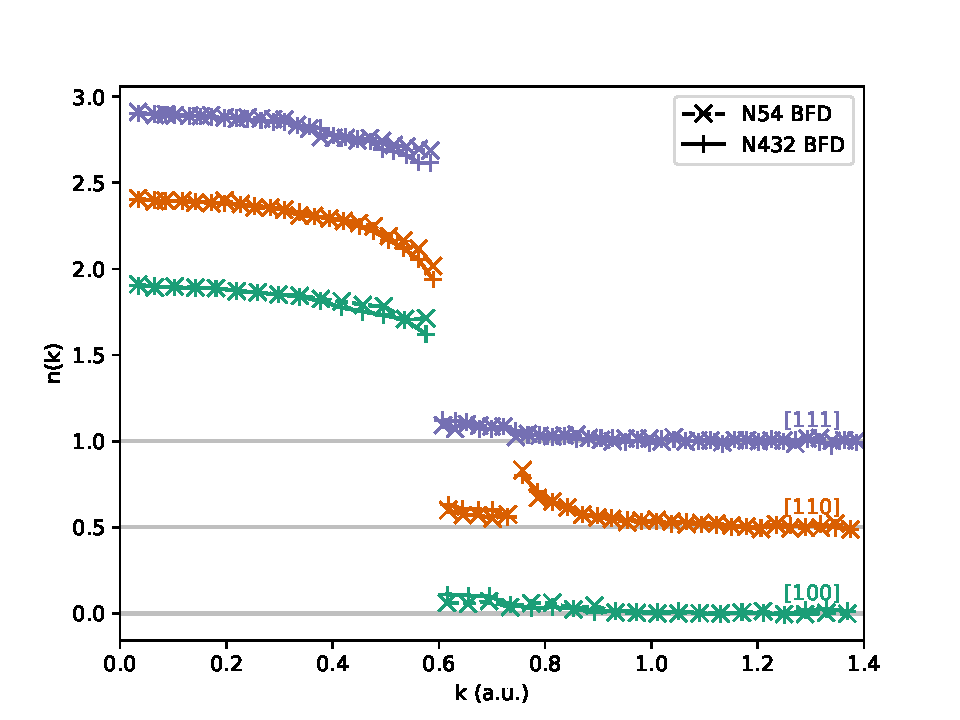
\includegraphics[width=\linewidth]{li52g_bfd-crystal-n54-n432-nk}
(b) 432 atoms \textit{vs} 54 atoms
\end{minipage}
\caption{Momentum distribution of valence electrons in lithium BCC crystal. The top panel compares pseudopotential (crosses) to full-core (dots) result.
The bottom panel compares 54-atom (crosses) to 432-atom (pluses) pseudopotential results.\label{fig:nk}}
\end{figure}

In Fig.~\ref{fig:dnk}, we show two sets of momentum distribution differences in direct correspondence with Fig.~\ref{fig:nk}. The first is the difference between full-core and pseudopotential momentum distributions. This difference can be considered a pseudopotential correction (PPC). The PPC is largest inside the Fermi surface. It has a parabolic shape and is mostly negative along the [100] and [111] directions. However, it shows positive peaks near the secondary Fermi surface along the [110] direction.  The PPC is spherically-averaged and applied to the momentum distributions of the disordered structures.

Now consider how the finite size of our supercell affects the results: the finite-size correction (FSC). The bottom panel of Fig. Fig.~\ref{fig:dnk} show the changes between the 432-atom and 54-atom pseudopotential calculations. The difference peaks at the Fermi surface and goes to zero at high momenta.  The FSC results shown here are used it to validate the approach outlined in ref.~\cite{Holzmann2009} and ref.~\cite{Holzmann2011}.

\begin{figure}
\begin{minipage}{\columnwidth}
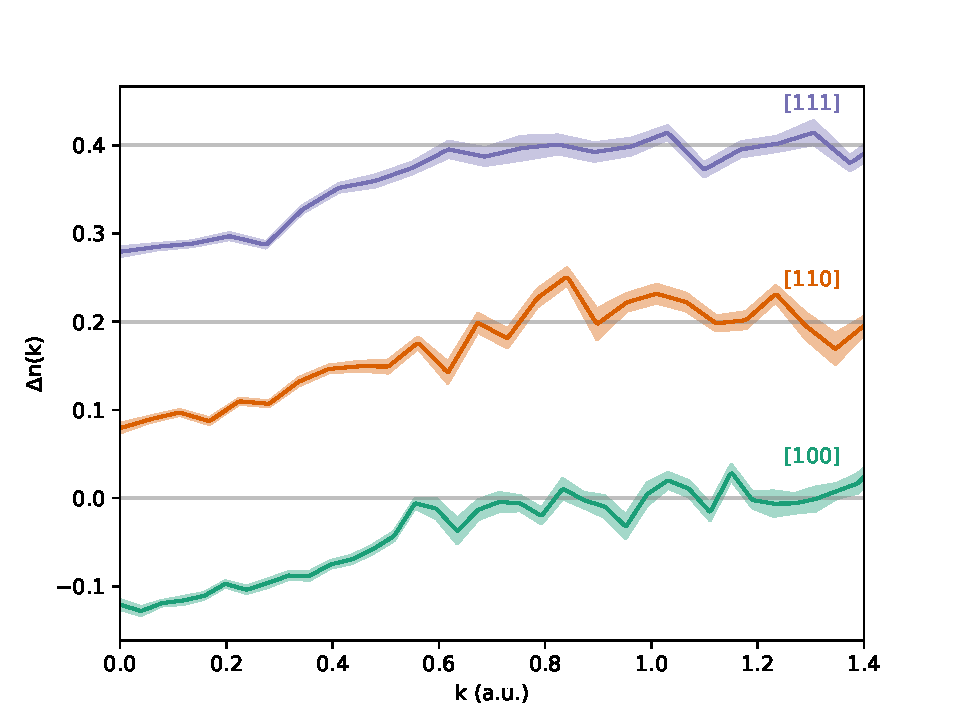
\includegraphics[width=\linewidth]{li57_dmcfc-ppc-dir}
(a) full-core valence - pseudopotential
\end{minipage}
\begin{minipage}{\columnwidth}
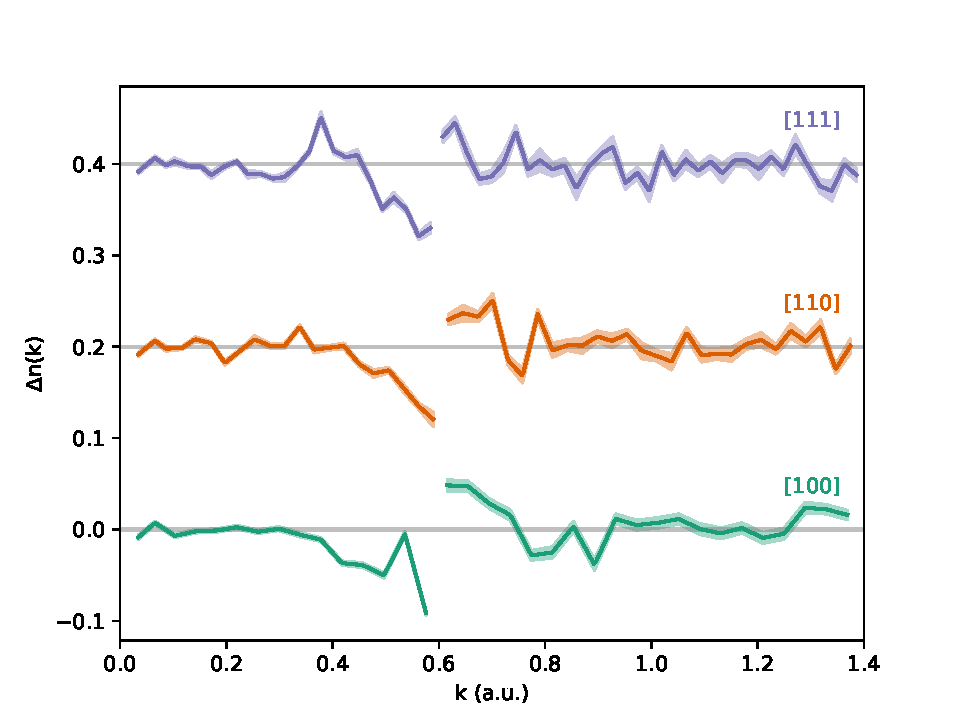
\includegraphics[width=\linewidth]{li52g_bfd-crystal-n54-n432-dnk}
(b) 432 atoms - 54 atoms
\end{minipage}
\caption{Momentum distribution differences. The top panel is the difference between full-core and pseudopotential results. The bottom panel is the difference between the 432-atom and 54-atom pseudopotential results. The shaded region show one standard deviation of statistical uncertainty. These results are used to inform pseudopotential and finite-size corrections. \label{fig:dnk}}
\end{figure}

In Fig.~\ref{fig:crystal-vcp}, we show our best QMC Compton profile in the crystal as the red line. It is the spherically-averaged Compton profile from the 432-atom pseudopotential calculation with PPC and FSC applied. Further, we rescaled the QMC data to change density from $r_s=3.25$ to $r_s=3.265$ and convolved the QMC Compton profile with Eq.~(\ref{eq:elorentz}) to approximately account for experimental resolution and final state effects. The full-core QMC profiles agrees well with the most recent experiment away from the Fermi surface.

The Compton profile reported by Filippi and Ceperley \cite{Filippi1999} is closer to our full-core than to our pseudopotential result. This is because they accounted for proper core-valence orthogonalization using full-core LDA. Pseudopotential QMC was used to estimate the correlation correction, rather than directly provide the Compton profile.
%their reported QMC Compton profile effectively includes an LDA pseudopotential correction. Specifically, full-core LDA + QMC correlation correction = pseudopotential QMC + LDA pseudopotential correction.

\begin{figure}
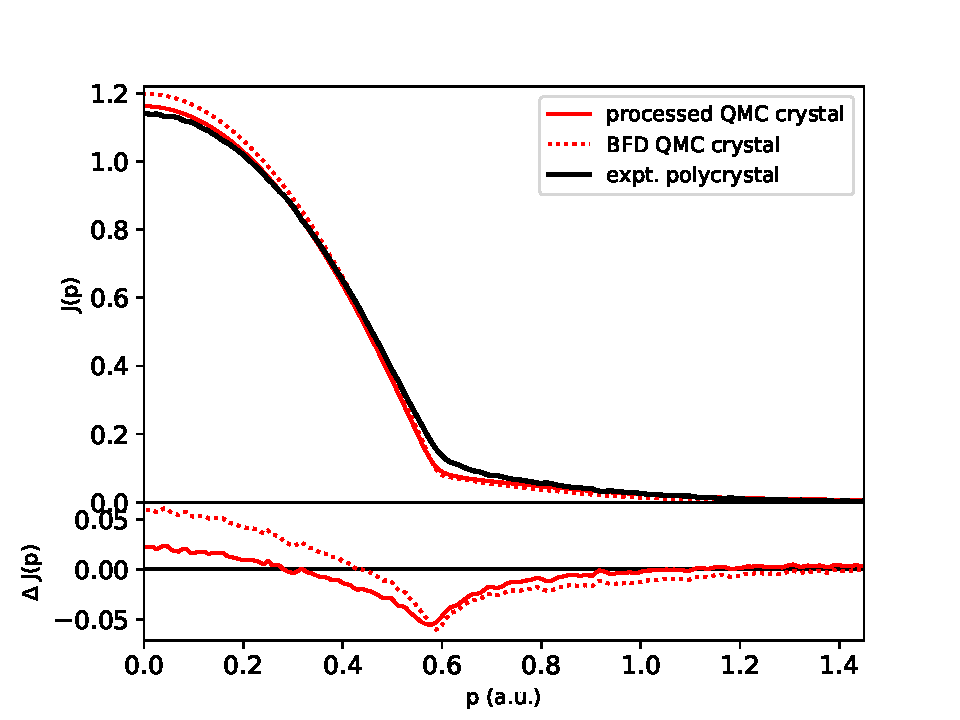
\includegraphics[width=\linewidth]{li62g_crystal-jp}
\caption{Spherical average of the valence Compton profile of lithium BCC crystal at $r_s=3.25$. The red solid line is the best QMC result with all processing steps applied. The red dotted curve is our pseudopotential QMC result. The black curve is experiment on polycrystal lithium. \label{fig:crystal-vcp}}
\end{figure}

Taking our best QMC Compton profiles (colored line in Fig.~\ref{fig:sl-jp-djp}) as reference, we show the remaining difference between the QMC and the experiment Compton profiles as the black curves in Fig.~\ref{fig:sl-corrections}. We also show the effect of each processing step in the calculation of $J(p)$. %As shown in Fig.~\ref{fig:crystal-ppc}, three corrections are considered: pseudopotential, finite-size, and convolution. All three lower the value of $J(0)$, bringing it closer to experiment. The pseudopotential correction is dominant over the convolution and finite-size corrections. Further, the pseudopotential correction is the only one that contributes at momenta far above the Fermi momentum ($p>0.75$ a.u.).

\begin{figure}
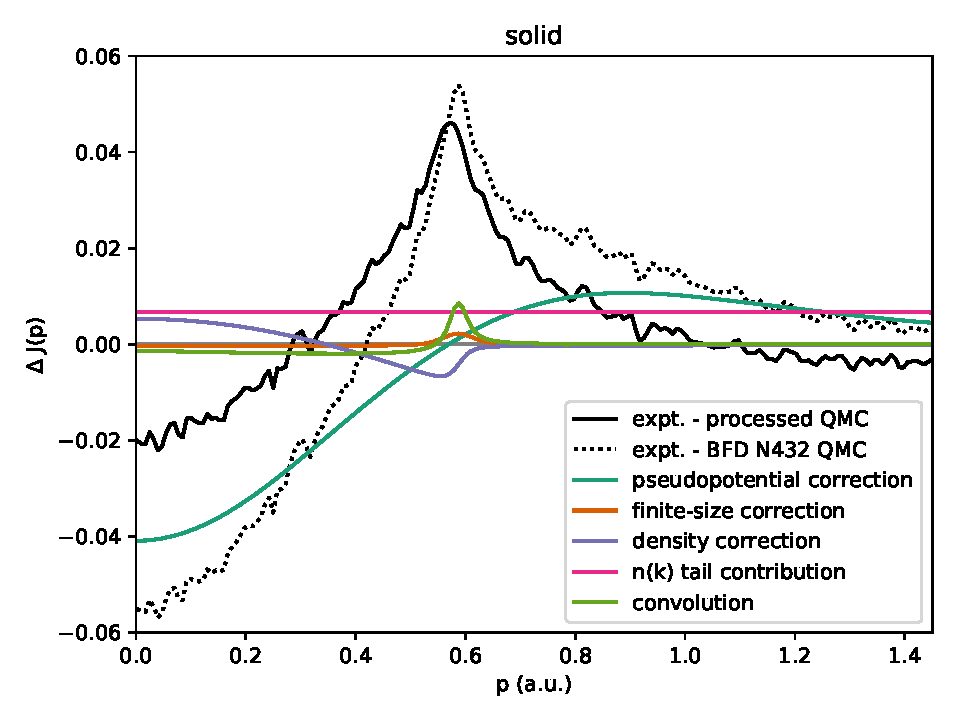
\includegraphics[width=\linewidth]{li58_solid-the-djp}
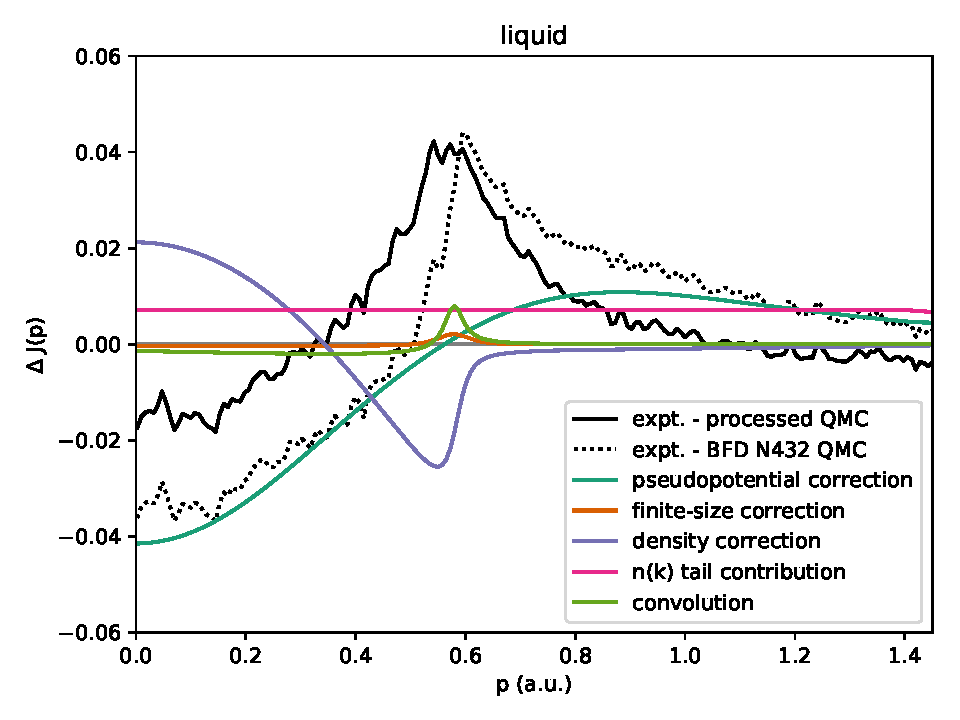
\includegraphics[width=\linewidth]{li58_liquid-the-djp}
\caption{Compton profile corrections. The solid black curve is experiment relative to ``best'' theory. The dotted black curve is experiment relative to pseudopotential QMC result with no correction. The colored curves are various corrections to the theoretical Compton profile. \label{fig:sl-corrections}}
\end{figure}

\section{Discussion} \label{sec:discussion}

In the following, we discuss possible explanations for the remaining discrepancy in Fig.~\ref{fig:sl-jp-djp}. %The possibilities can be grouped into two conceptual categories: 1. imperfect inclusion of an effect we have considered; 2. the omission of an effect we have not considered. In the first category, we have considered correlation, thermal disorder, finite-size, and final-state interaction. In the second category, we have not considered the effect of thermal expansion, electronic thermal excitation, relativistic effects, and changes in the shape and location of the Fermi surface.

{ \bf Electron-Ion interaction} The crystal lattice introduces inhomogeneity to an otherwise homogeneous valence electron density. Umklapp processes send electronic momentum density to secondary Fermi surfaces, thereby enhancing the high-momentum components of the momentum distribution and reducing the momentum distribution inside the Fermi surface. Further, its discontinuity at the Fermi surface is reduced~\cite{Eisenberger1972}.
In the absence of other interactions, the ground-state electronic density will be exact if the electron-ion interaction is perfectly captured. DFT is designed to obtain the correct ground-state electronic density, so we expect it to treat electron-ion interaction well. However, pseudopotential is not designed to faithfully reproduce the charge inhomogeneity of the valence orbital in the core region. Therefore, pseudopotential introduces a bias in the valence momentum distribution.

The qualitative effect of the pseudopotential is clear from its construction. When designing a pseudopotential, one smooths the valence orbital inside the core region. This will decrease the electronic momentum density at high momenta, and increase it at low momenta. Indeed, one can reproduce the pseudopotential correction semi-quantitatively by considering the smoothing of the pseudized valence orbital in the lithium atom (Fig.~\ref{fig:hf-ppc}). We see that augmented planewave (APW) calculations~\cite{Baruah1999,Bross2004,Bross2005,Bross2012} tend to reproduce the experimental Compton profiles better at low momenta than pseudopotential calculations.

\begin{figure}
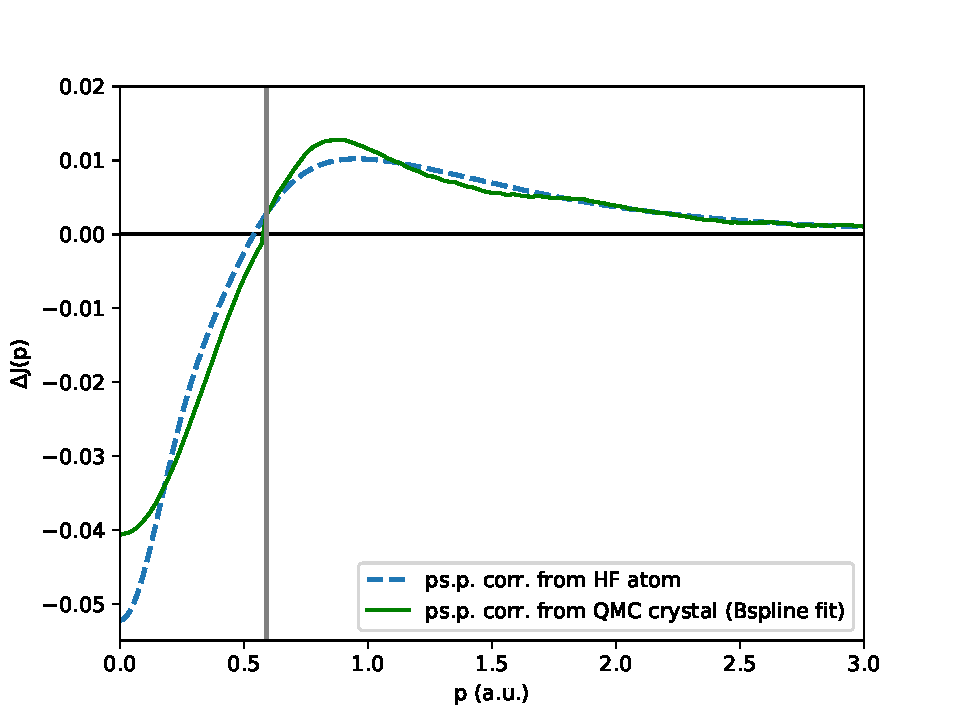
\includegraphics[width=\linewidth]{li42c_bfd-dmcppc}
\caption{Pseudopotential correction derived from QMC and HF. The green curve is the same QMC pseudopotential correction as shown in Fig.~\ref{fig:sl-corrections}. The dashed blue curve is the pseudopotential correction derived from the all-electron v.s. pseudized lithium atom using HF. The gray vertical line marks the Fermi momentum. \label{fig:hf-ppc}}
\end{figure}

Our pseudopotential correction (PPC) is not perfect. It was derived in the perfect crystal, then applied to the disordered configurations. Ideally, one would directly perform all-electron QMC on the disordered configurations. However, this is computationally expensive. We do not consider all-electron calculation to be necessary in the solid phase, because the effect of disorder is small. The current PPC does over correct the liquid Compton profile at high momenta, because the corrections meant for the secondary Fermi surfaces are extraneous. Nevertheless, we think the pseudopotential bias is mostly captured, i.e. at the scale of Fig.~\ref{fig:hf-ppc}. The corrected Compton profile in Fig.~\ref{fig:crystal-vcp} is in better agreement with experiment than its pseudopotential counterpart, especially at $p=0$. We do not think the pseudopotential bias is responsible for the remaining discrepancy, because the PPC is concentrated around $p=0$. If it were underestimated, then the remaining correction would lower $J(0)$ much more than it would raise $J(p_F)$, worsening the agreement with experiment. %Therefore, we think electron-ion correlation has been satisfactorily accounted for, and is not responsible for the remaining discrepancy.

{\bf Disorder}  Disorder mostly reduces the effect of the crystal lattice, because deviations from the perfect lattice weakens Umklapp processes. A confirmation was obtained when Sternemann et. al. reproduced the temperature effect on the Compton profile of lithium by smearing out the pseudopotential with a Debye-Waller factor~\cite{Sternemann2001}.

Thermal disorder is also unlikely to be responsible for the remaining discrepancy because disorder-correction is small at the scale of the remaining correction. This can be seen by comparing the discrepancy in the perfect crystal (Fig.~\ref{fig:crystal-vcp}) to the discrepancy in the disordered solid (Fig.~\ref{fig:sl-jp-djp}). The two remaining discrepancies are similar in both shape and magnitude.

%Thermal disorder and thermal expansion can also contribute to the remaining discrepancy. The main effect of thermal disorder is to smear out the reciprocal lattice and suppress Umklapp processes~\cite{Sternemann2001}. This transfers electron momentum density from the secondary Fermi surfaces back to the main one, thus narrowing the Compton profile.

{\bf Electron-Electron Correlation}  The effect of electron-electron (ee) correlation on the momentum distribution is similar to electron-ion interaction in that it increases high-momentum components, decreases low-momentum components and reduces the discontinuity at the Fermi surface. %However, electron-electron correlation does not introduce secondary Fermi surfaces.
%While the LDA functional encodes ee correlation, it is completely absent from the KS determinant wavefunction. 
The Slater-Jastrow wavefunction is a first-order modification of the free-electron Slater determinant by the Coulomb interaction~\cite{Holzmann2003} %Therefore, the Slater-Jastrow wavefunction captures correlation in a rigorous and rather natural manner. 
but it does not capture all correlation effects. 
% and puts a bias on the DMC momentum distribution due to fixed-phase error and mixed-estimator bias. 
However, we expect the Slater-Jastrow wavefunction to be accurate for simple metals. 
Further, it can be systematically improved, for example by using backflow transformations \cite{PhysRevB.91.115106}. 
\mh{Calculations on the homogeneous electron gas indicate a small decrease of the discontinuity
at the Fermi 
surface \cite{Holzmann2011} reducing the discrepancy with experiment. Quantitive studies of
backflow effects on the lithium Compton profiles should be adressed in future.}
%The change in going from the variational to mixed estimator provides an estimate of missing corelation effects. \david{how big is this?}
%Going to second order, we have back flow correlation as well as three-body Jastrow.

%Remaining ee correlation effect is unlikely to be the main cause of the remaining discrepancy because the isotropic Lam-Platzman correction derived from the homogeneous electron gas was shown to be accurate by QMC~\cite{Filippi1999,Bross2005}. Further, the correlation correction of the LDA Compton profile is a relatively smooth function of momentum with a peak of magnitude $\sim$0.05 a.u. at the Fermi momentum. It seems unlikely that the remaining correlation correction to the QMC Compton profile would be of the same magnitude.

%Bross found that the Lam-Platzman correction is sensitive to the underlying model of the homogeneous electron gas~\cite{Bross2005}.

{\bf Electron-phonon interaction} Phonons are \mh{partially} absent from our QMC simulations because the lithium ions are clamped. Phonons scatter quasi-particles and decrease their life times. Thus, we expect the inclusion of electron-phonon interaction to decrease the magnitude of the discontinuity in the momentum distribution. \mh{Calculations of the coupled electron-phonon system within the Einstein or Debye model \cite{PhysRev.131.993}, shows that the resulting  broadening
at zero temperature is essentially given by the Debye frequency.}
However, the Debye temperature of lithium ($<$400K) is much lower than the Fermi temperature of the electrons, so we expect the effect of the \mh{remaining} electron-phonon coupling \mh{not included
in our QMC calculations} to be limited very close to the Fermi surface in momentum space, rendering the effect invisible at the scale of Fig.~\ref{fig:s-l-djp}.


{\bf Finite size effects}  Finite-size effects (FSE) are more challenging to deal with in a many-body simulation than in an effective one-particle theory such as DFT which is formulated for an infinite lattice. A calculation performed in a larger simulation cell simply makes the momentum-space grid denser. In contrast, finite system size increases the magnitude of the discontinuity at the Fermi surface in QMC. This effect was found to decrease slowly with system size in the homogeneous electron gas~\cite{Holzmann2009}. This FSE  was analyzed and understood in the homogeneous electron gas~\cite{Holzmann2009,Holzmann2011}. We adopted the same approach here and found good results. In particular, we corrected the FSE using the leading-order expression
\begin{equation} \label{eq:nk-fsc}
\delta n_{\bs{k}}^{(1)} = \int_{-\pi/L}^{\pi/L} \frac{d^3\bs{q}}{(2\pi)^3} \left[
u_q (1-S_q) - nu_q^2 S_q
\right] (n_{\bs{k}+\bs{q}}-n_{\bs{k}}),
\end{equation}
where $u_q$ and $S_q$ are the Jastrow pair function and the structure factor in reciprocal space, which are assumed to take RPA forms at small $q$ and $n$ is the valence electron density. The corrected $n(k)$ from the 54-atom and 432-atom simulations agree well with each other as shown in Fig.~\ref{fig:liquid-nk-fsc}. Therefore, we think finite-size error has been satisfactorily accounted for, and is not responsible for the remaining discrepancy.

\begin{figure}
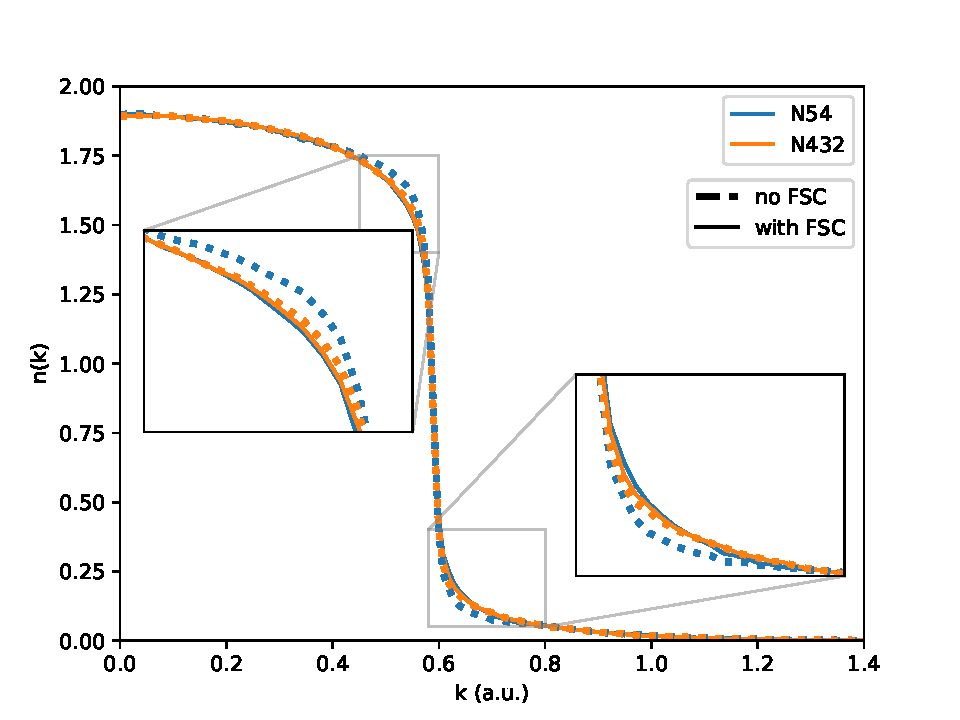
\includegraphics[width=\linewidth]{li58h_liquid-fsc}
\caption{Finite-size correction in the liquid phase. Dotted lines are pseudopotential QMC $n(k)$ with no correction. Color encodes the number of lithium atoms in the simulation cell. The solid lines correspond to the dotted lines in color and have been corrected using the leading-order expression Eq.~(\ref{eq:nk-fsc}). \label{fig:liquid-nk-fsc}}
\end{figure}

{\bf Density change} The electronic density is a crucial parameter since it determines the Fermi surface. It can change due to thermal expansion and phase transition from solid to liquid .%E. Klevak et. al. showed that upon raising temperature from 0 to 300K, the Compton profile narrows and $J(0)$ increases by $\sim$ 0.025 a.u.~\cite{Klevak2016}. The experimental Fermi momenta for the solid and liquid states are 0.595 and 0.585 a.u., respectively. They correspond to homogeneous valence densities of $r_s=3.225$ and $r_s=3.28$, which differ slightly from the density $r_s=3.25$ used in our calculations.
We accounted for density change between our calculations and experiment by rescaling our computed momentum distributions to the experimental densities by scaling the value of $k$ to match the Fermi momentum ($k_F=(9\pi/4)^{1/3}/r_s$) and then correcting the overall normalization.
%To rescale, we first put $n(k)$ in unitless form $\tilde{n}(x)$, where $x\equiv k/k_F$ and $\tilde{n}(x)\in[0, 1]$. \david{Does this preserve the sum rule?} Then, we use the experimental density to calculate momentum and the normalization constant of the Compton profile using . 
This brought the Compton profile into excellent agreement with experiment as shown in Fig.~\ref{fig:s-l-djp}.  Of course it would be possible to perform additional QMC simulations at the experimental density. %Therefore, we think density change has been satisfactorily accounted for, and is not responsible for the remaining discrepancy.

{\bf Fermi surface}  The Fermi surface of BCC lithium is anisotropic with pronounced secondary features. %The KS-LDA main Fermi surface is a mesh of octagons facing [100], [110], triangles facing [111], and square patches to close the surface. The whole surface curves to approximate a sphere, somewhat like a soccer ball. Further, there is a clear secondary Fermi surface along the [110] direction at $p=(0.6, 0.6, 0)$ a.u..
The DFT Fermi surface is used in the QMC simulation to determine which momentum states to occupy.
For solid lithium the Fermi surface is nearly spherical \david{can we find de Haas -Van Alphen data on the non-spherical parameter and compare to DFT?} 
\mh{Our inclusion of thermal configurations leads to a broadening of the Fermi surface, washing out
any small differences between DFT and the exact one.}
While the DFT Fermi surface may not be accurate in the crystal,  a liquid is isotropic and will have a spherical Fermi surface.
Given that our liquid - solid Compton profile difference agrees well with experiment (Fig.~\ref{fig:s-l-djp}), we do not consider Fermi surface shape to be responsible for the remaining discrepancy.


{\bf Final state effects} Finally, the ``impulse approximation'' is known to be inaccurate for core electrons and cause asymmetry in the measured Compton profile~\cite{Eisenberger1970,Sternemann2000,Huotari2001}. To go beyond the ``impulse approximation'', one must consider interaction of the scattered electron with the rest of the system in the final state. Final-state effects are often attributed to three physical interactions. The first is the interaction between the excited quasi-particle with its surrounding medium. The second is the interaction between the excited quasi-particle and the hole it lefts behind (vertex correction). The third is the interaction between the hole and a plasmon (plasmaron). C. Sternemann et. al. showed that the self-energy combined with the vertex correction can satisfactorily explain the asymmetry of the Compton profile~\cite{Sternemann2000}. The effect of final-state interaction on the Compton profile can be approximated by convolving the spectral density function of the excited electron with the ground-state Compton profile~\cite{Soininen2001}. This convolution smears out the derivative-discontinuity of the Compton profile at the Fermi momentum. Thus the convolution correction also peaks at the Fermi momentum.

We account for final-state effects by convolving the QMC Compton profiles with the broadening function Eq.~(\ref{eq:elorentz}), which is an accurate representation of the convolution of the experimental resolution function and the spectral density function (SDF) from ref.~\cite{Soininen2001}. However, the SDF in ref.~\cite{Soininen2001} did not include plasmaron or electron-hole effects. Further, we find near perfect agreement with experiment if the QMC profiles were broadened using a Lorentzian having FWHM $\Gamma=0.026$. In other words, if the neglected final-state effects were to introduce long tails into the SDF, then the QMC profiles would agree much better with experiment. Therefore, final-state effect is a plausible explanation for much of the remaining discrepancy.

%Final-state effect is unlikely to be the main cause of the remaining discrepancy, because the convolution correction is small on the scale of the discrepancy shown in Fig.~\ref{fig:sl-corrections}. Further, the convolution correction is insensitive to small adjustment of parameters in the model function.

%We found that if the pseudopotential QMC Compton profiles were convolved with a Lorentzian having FWHM $\Gamma=0.026$ a.u., then they would agree almost perfectly with experiments. We believe this agreement is rather fortuitous. The long tail of the Lorentzian happens to be able to model the effect of the pseudopotential at $p=0$ and the remaining smearing at $p=p_F$ simultaneously.

% hypothesis: the slow varying background is due to the failure of the IA. The peak at Fermi momentum is due to remaining correlation and finite-size errors.

\section{Conclusion and Outlook}

Leveraging new algorithms and hardware, we improved the QMC Compton profile of lithium and provided the first QMC results in the disordered solid and the liquid states. Our QMC Compton profiles of the disordered solid and the liquid agree very well with the most recent synchrotron experiment. We resolved the discrepancy between pseudopotential QMC and experiment at zero and high momenta using an all-electron QMC calculation. We discussed potential explanations for the remaining discrepancy, which is concentrated at the Fermi surface. Future studies should consider final-state effects.

Current state-of-the-art QMC algorithms are ready to aid synchrotron experiments in understanding the measured Compton profiles. It would be interesting to revisit the challenging problem that is the 3D reconstructing of the momentum distribution from directional Compton profiles~\cite{Schulke1996,Tanaka2001}. Momentum resolution has been increased by new techniques in both theory and experiment. Further, all-electron QMC for lithium is feasible for perfect crystals in supercells containing thousands of electrons. The comparison between lithium and sodium will be particularly interesting, because they have the same crystal structure but very different electron-ion interactions~\cite{Eisenberger1972}. A detailed study of these systems can shed more light on the nature of electron-ion and perhaps the electron-phonon interactions in simple metals.

Finally, when sufficient accuracy has been achieved in both theory and experiment, one can study the difference between ground-state (QMC) and final-state (experimental) Compton profiles to extract information on the dynamic structure factor of the system.

\section{Acknowledgment}

YY and DMC were funded by DOE 0002911. This work made use of the Blue Waters sustained-petascale computing project and the Illinois Campus Cluster, supported by the National Science Foundation (awards OCI-0725070 and ACI-1238993), the state of Illinois, the University of Illinois at Urbana-Champaign and its National Center for Supercomputing Applications.
%We would like to thank Kazuhiro Matsuda and Nozomu Hiraoka for sharing their experimental Compton profiles with us.
We would like to thank Ilkka Kyl\"anp\"a\"a and Jaron Krogel for valuable discussions.

\bibliographystyle{apsrev4-1}
\bibliography{ref}

\end{document}
